\chapter{Despliegue por defecto.} \label{cap:02Despliegue}

El despliegue de ATLAS en Docker es muy sencillo y está muy bien documentado en su repositorio de github  \cite{githubBroadsea}.  Igualmente, en este manual se detallan nuevamente los pasos para la configuración y despliegue de la herramienta, añadiendo algunos pasos relevantes adicionales.

\section{Requisitos para el despliegue} \label{sec:02requisitos}

\begin{enumerate}
    \item Descargar e instalar Docker. Lo más sencillo es seguir las instrucciones de la \href{https://docs.docker.com/engine/install/}{página web oficial} para la descarga y seguir la configuración por defecto para la instalación.
    
    \item Descargar e instalar Git. Lo más sencillo es seguir las instrucciones de la \href{https://git-scm.com/downloads}{página web oficial} para la descarga y seguir la configuración por defecto para la instalación.
\end{enumerate}

\section{Deployment} \label{sec:02Deployment}

En este primer despliegue rápido de ATLAS, se desplegarán las configuraciones por defecto de la herramienta, siguiendo la guía de implementación rápida \textit{(Quick Start)} del mismo repositorio de github.

\begin{enumerate}
    \item Por tanto, el primer paso para desplegar ATLAS es clonar localmente el repositorio de github de Broadsea. Una forma rápida de hacerlo es copiar la siguiente línea de código en el \code{cdm}.

\begin{lstlisting}[language=sh]
        git clone https://github.com/OHDSI/Broadsea.git
\end{lstlisting}

    \item El segundo paso, es desplegar el contenedor docker. Para ello, situar el puntero del \code{cdm}, en la carpeta donde se ha copiado el repositorio de github de Broadsea.

\begin{lstlisting}[language=sh]
        cd ruta\del\repositorio\Broadsea\local
\end{lstlisting}

    Una vez situado en la carpeta raíz del repositorio, se jecuta el comando que instalará y desplegará el perfil por defecto del contenedor docker en la máquina local.

\begin{lstlisting}[language=sh]
    docker compose pull && docker-compose --profile default up -d
\end{lstlisting}

\end{enumerate}

\section{Comprobación de despliegue correcto} \label{sec:02comprobacion} 

Se puede comprobar que se ha instalado correctamente el contenedor de Broadsea en la máquina local de distintas formas, tal y como se presenta a continuación.

\begin{enumerate}[label=\alph*]

    \item \textbf{Comprobación a través de Docker Desktop.} La forma más sencilla de interactuar con el contenedor de Broadsea es a través de Docker Desktop. Ejecutando dicho programa, en la sección \textit{''containers"} se muestran todos los contenedores que están corriendo en el equipo. En este caso, debe aparecer un multi-contenedor llamado "broadsea" que contenga seis contenedores, tal y como se muestra en la Figura \ref{fig:dockerDesktop} ''Captura de pantalla del contenedor Broadsea en Docker Desktop''.
    
\begin{figure}[H]
    \centering
    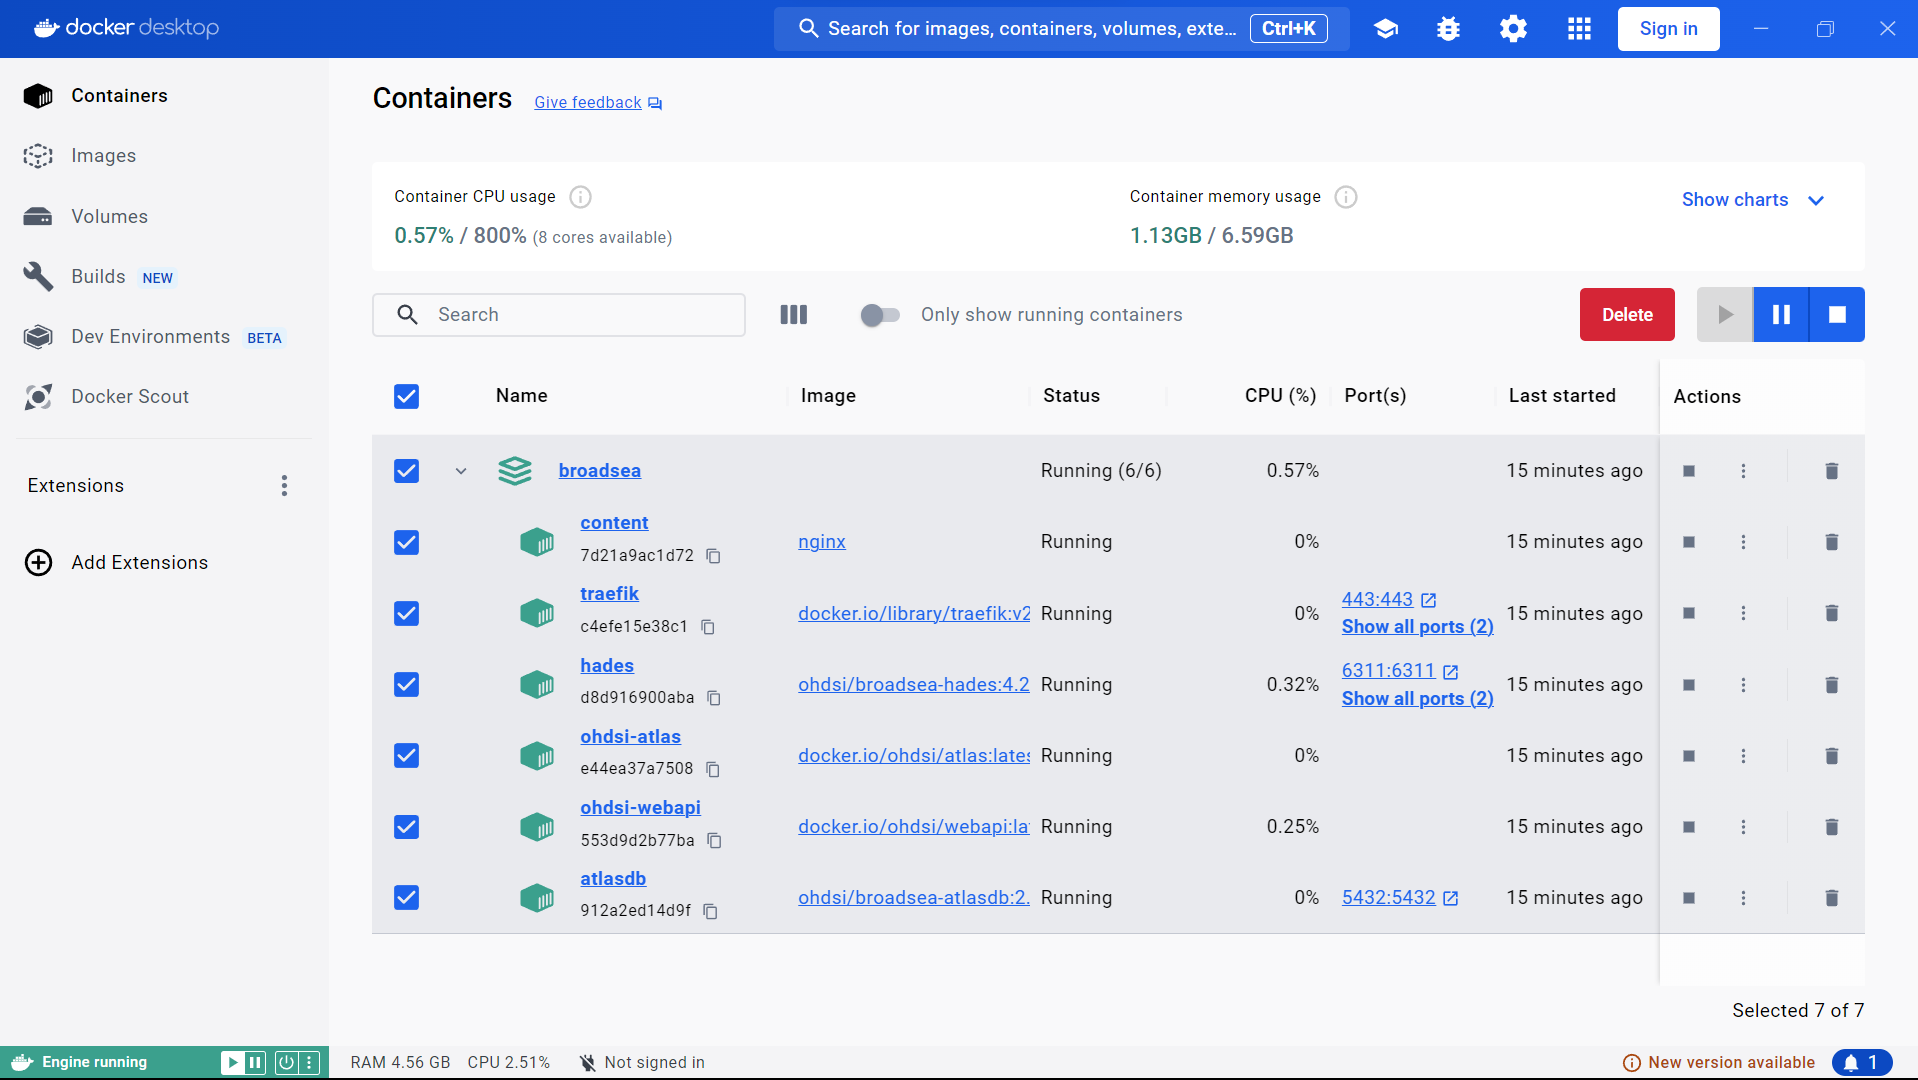
\includegraphics[width=0.90\textwidth]{figures/dockerDesktop.png}
    \caption{Captura de pantalla del contenedor Broadsea en Docker Desktop}
    \label{fig:dockerDesktop}
\end{figure}

    Mediante el panel de control de Docker se puede iniciar, pausar o detener cada contenedor (o todos a la vez) fácilmente y en cualquier momento. Por esto se dice que Broadsea ofrece servicios \textit{a-la-carte}.

    \item \textbf{Comprobación a través del \code{cmd}.} Otra forma de interactuar con el contenedor Docker es a través del \code{cmd}, ejecutando el comando \code{docker ps}, que muestra un listado de todos los contenedores que está ejecutando la máquina local. Con esta estrategia deberían mostrarse igualmente los mismos seis contenedores pertenecientes a broadsea, tal y como se muestra en la Figura \ref{fig:dockerCMD} ''Captura de pantalla del comando \code{docker ps } en el \code{cmd}''

\begin{figure}[H]
    \centering
    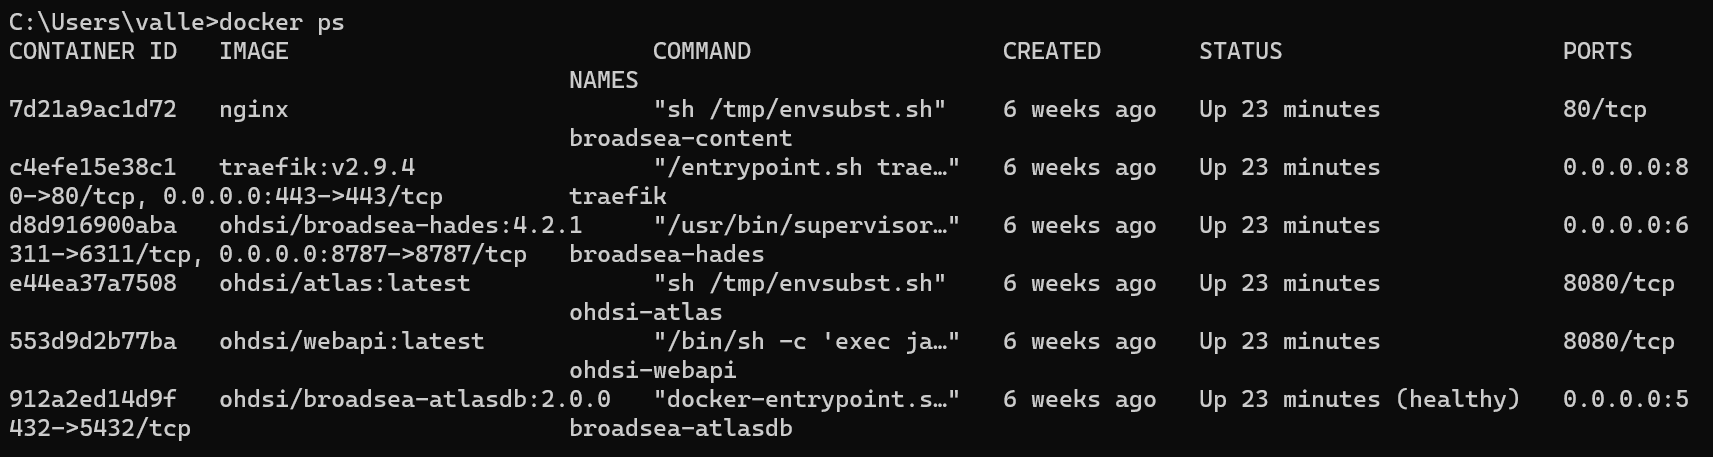
\includegraphics[width=0.90\textwidth]{figures/dockerCMD.png}
    \caption{Captura de pantalla del comando \code{docker ps } en el \code{cmd}}
    \label{fig:dockerCMD}
\end{figure}
    
    \item \textbf{Comrpobación a través del navegador.} Por último, para acceder a los servicios de Broadsea hay que abrir en el navegador web (Chrome recomendado) el servidor en el que se alojan los servicios. Por defecto, Broadsea se aloja en el servidor 127.0.0.1 (véase \ref{sec:01Postgre}).  Por tanto, introducir la dirección en el navegador para explorar las herramientas del contenedor, tal y como se muestra en la Figura \ref{fig:broadseaCap} ''Captura de pantalla del servidor Broadsea ejecutado en Chrome''.

    \begin{figure}[H]
    \centering
    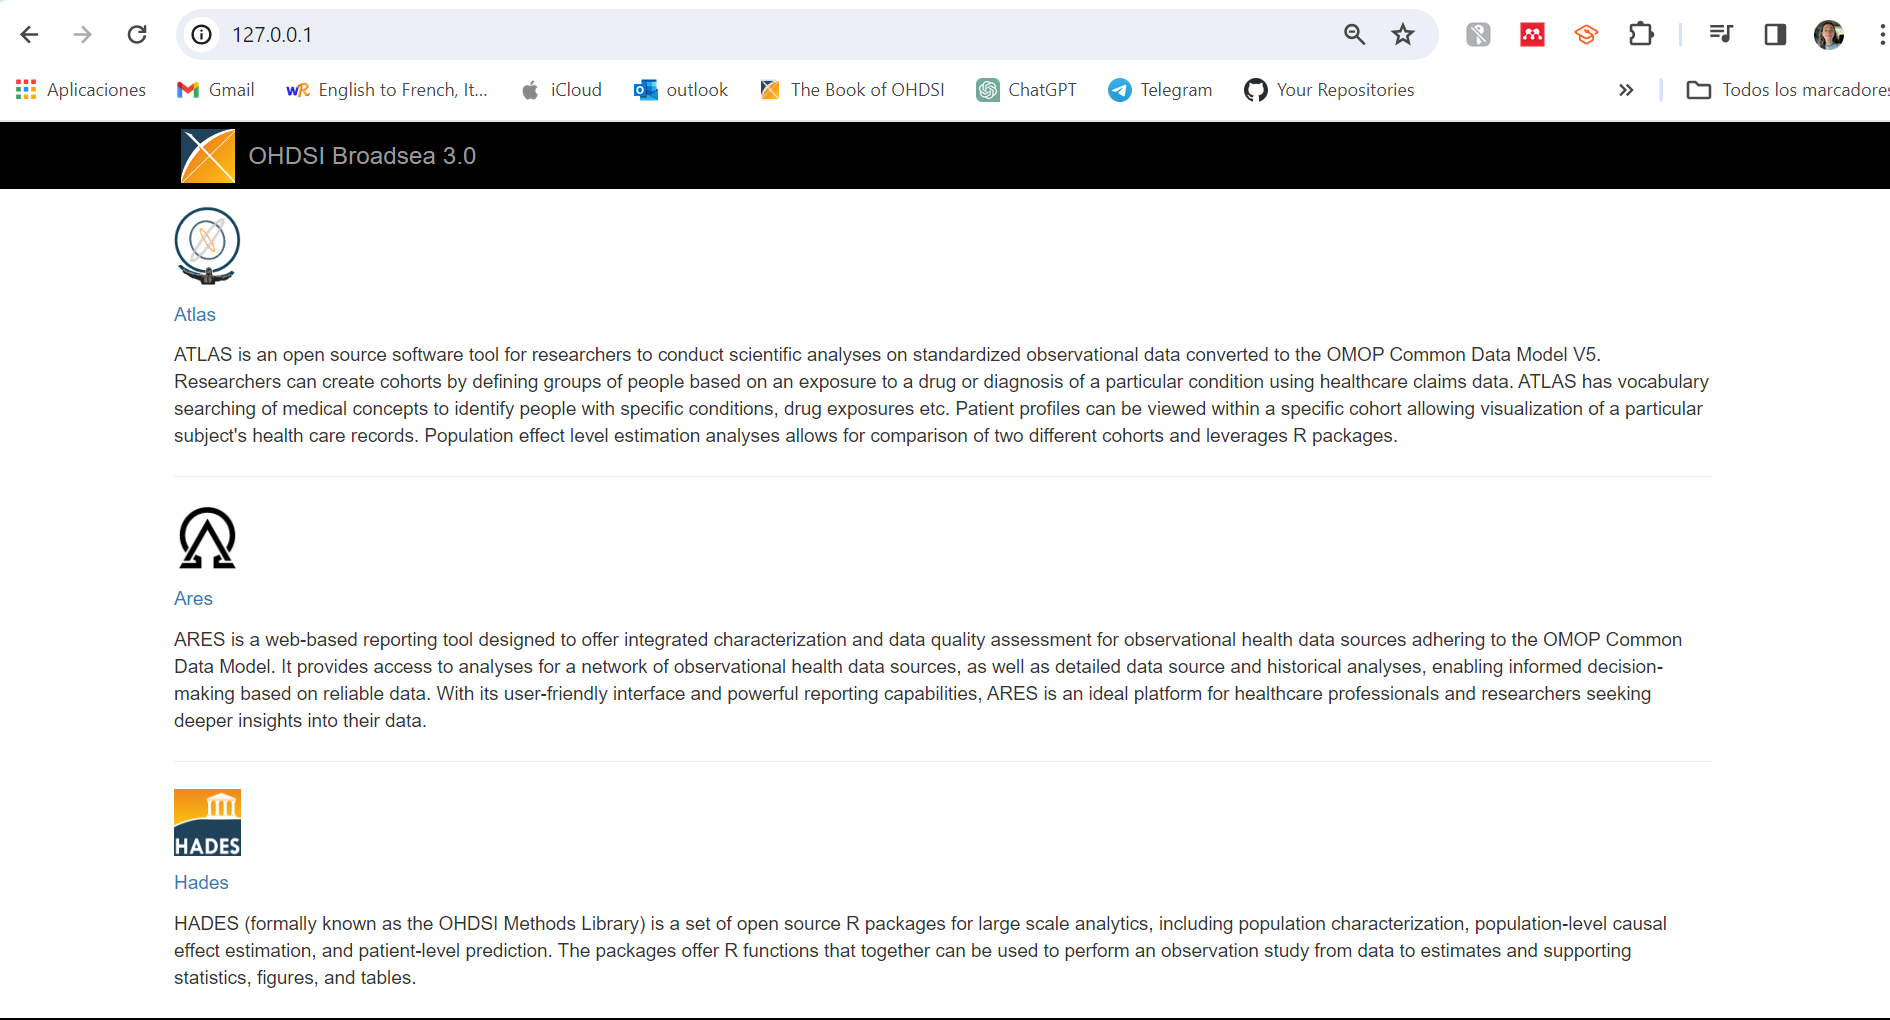
\includegraphics[width=0.90\textwidth]{figures/broadseaCap.png}
     \caption{Captura de pantalla del servidor Broadsea ejecutado en Chrome}
    \label{fig:broadseaCap}
\end{figure}
    
    Se puede comprobar o modificar el servidor exacto dónde se aloja el contenedor revisando el parámetro \code{BROADSEA\_HOST} de la sección 1 del archivo \code{.env} (para mayor información véase \ref{sec:01Docker} ''Entorno Docker de Broadsea'') de la ruta local del repositorio clonado . 

\begin{figure}[H]
    \centering
    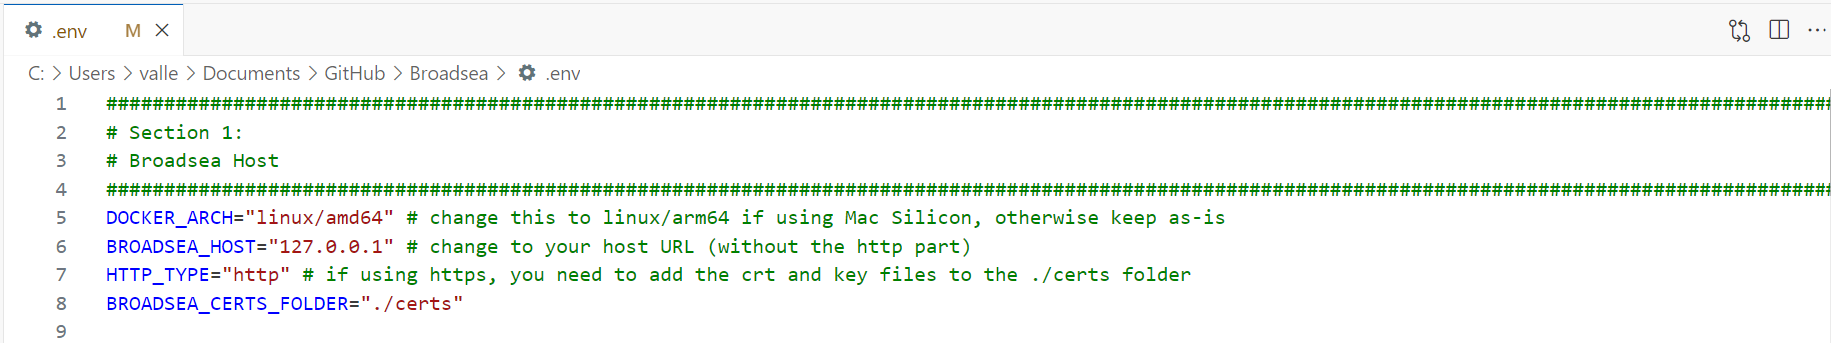
\includegraphics[width=0.90\textwidth]{figures/seccion1env.png}
    \caption{Captura de pantalla de la sección 1 del archivo \code{.env}.}
    \label{fig:seccion1env}    
\end{figure}

    En esta guía de implementación, no se va a modificar la dirección del servidor para la configuración de Broadsea, para no desconfigurar el entorno por defecto de la herramienta. Por tanto, el servidor de Broadsea durante todo el transcurso del manual será \code{127.0.0.1}, tal y como se recomienda en \cite{githubBroadseaDB} y como se muestra en la Figura \ref{fig:broadseaCap} ''Captura de pantalla del servidor Broadsea ejecutado en Chrome''

\end{enumerate}

    %Es interesante notar que Broadsea permite el acceso interactivo a la herramienta Atlas, que es la que nos interesa en este caso, pero también a Ares y a Hades, otras dos herramientas muy relacionadas (véase \ref{sec:01descripBroadsea} ''Descripción de Broadsea'').

    La ejecución de ATLAS en Broadsea es similar a ATLAS demo \cite{atlasDEMO}, aunque con algunas diferencias. En primer lugar, Broadsea solo ejecuta, por defecto, una base de datos, que es la base de datos de Eunomia (véase \ref{sec:01Postgre} ''Entorno PostgreSQL de Broadsea'').

\begin{figure}[H]
    \centering
    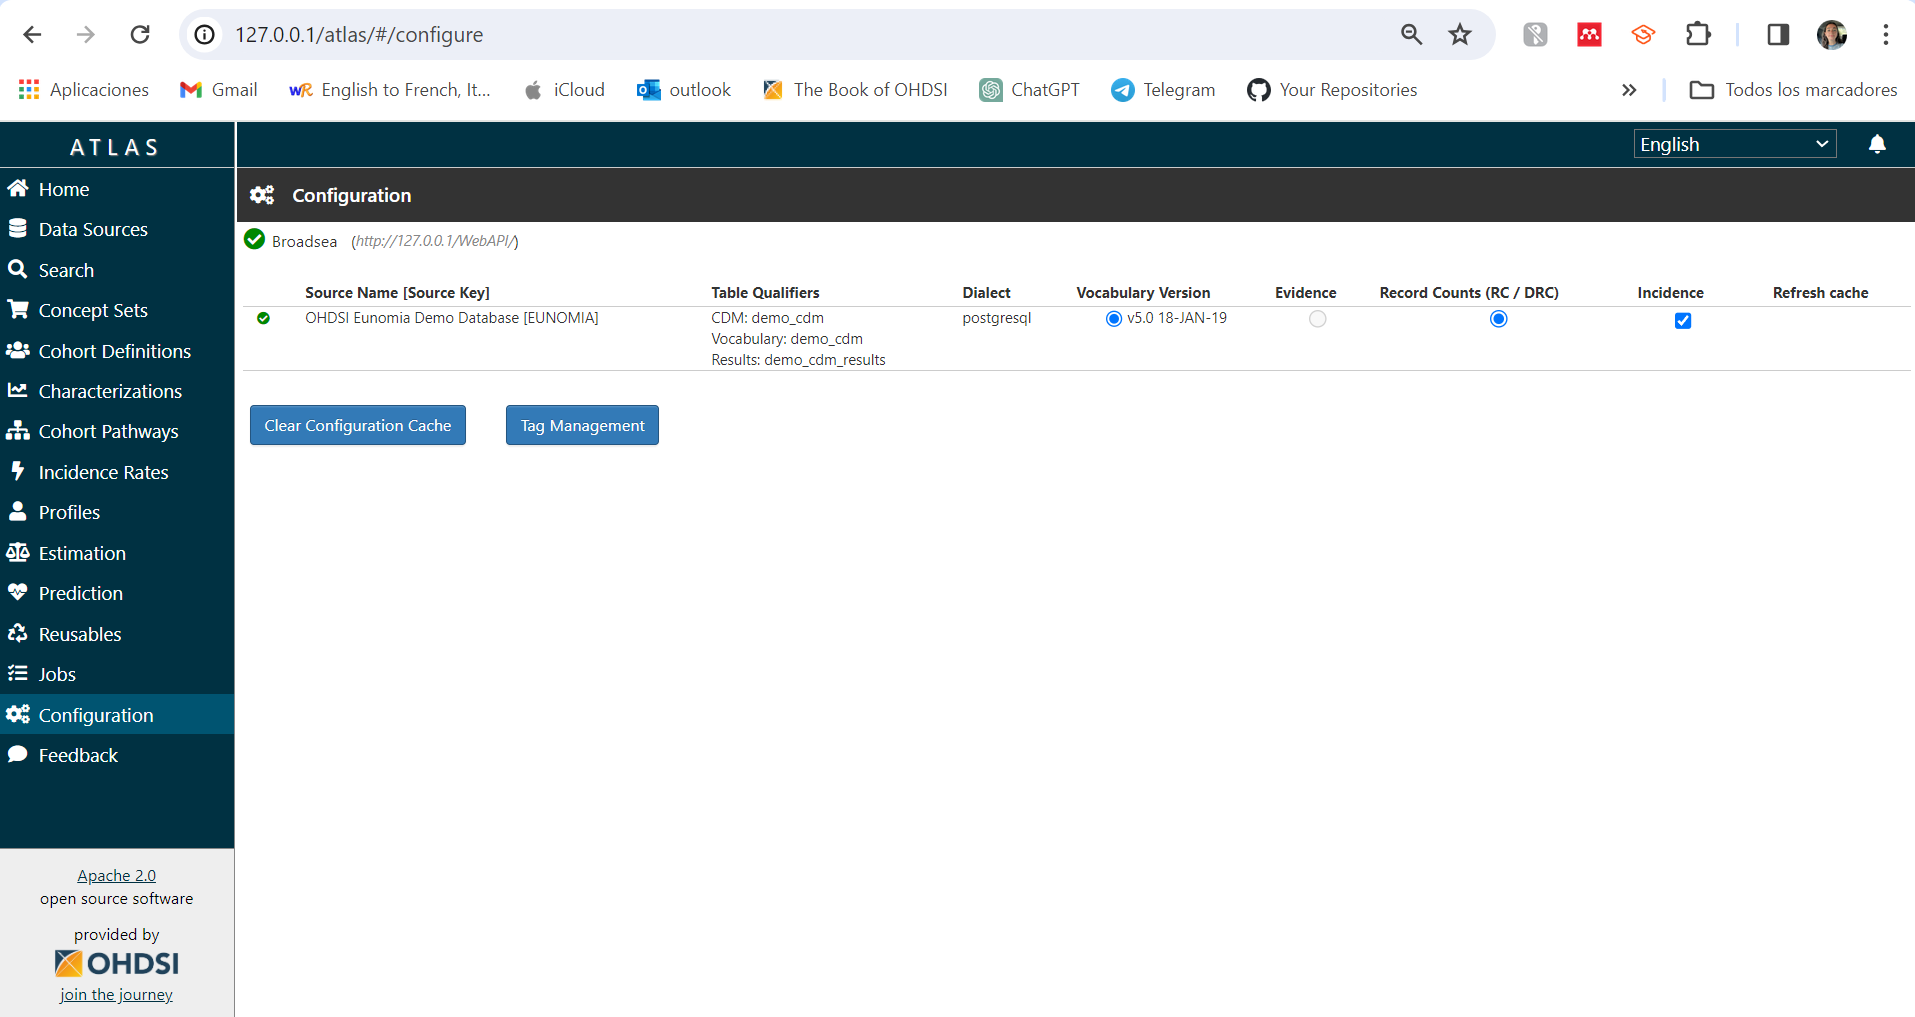
\includegraphics[width=0.90\textwidth]{figures/atlasBroadseaDB.png}
     \caption{Captura de pantalla de base de datos que utiliza ATLAS Broadsea}
    \label{fig:atlasBroadseaDB}
\end{figure}

    Por otra parte, y en contraste con la versión demo, ya no aparecen las entradas y estructuras que generan otros usuarios. La herramienta se presenta vacía, para ser completada solo con la información que el usuario local introduzca.

\begin{figure}[H]
    \centering
    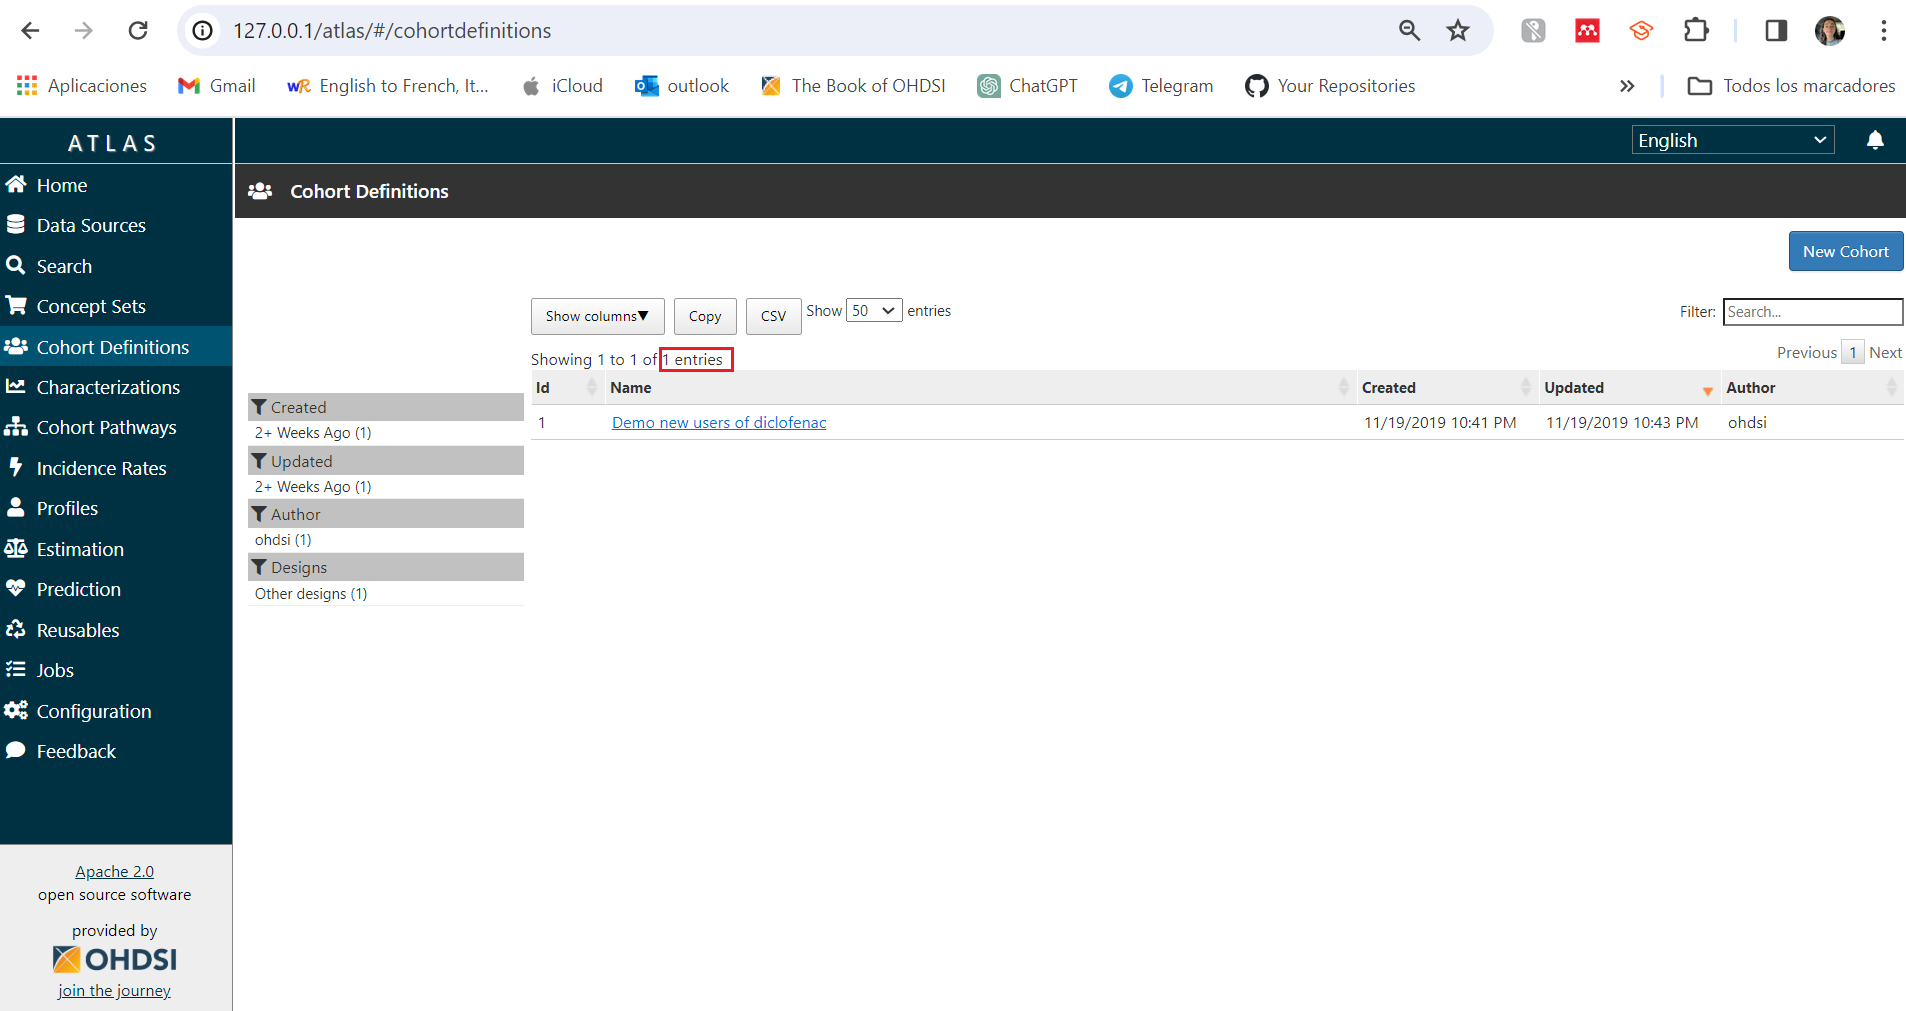
\includegraphics[width=0.90\textwidth]{figures/atlasBroadseaCD.png}
     \caption{Captura de pantalla señalando el número de entradas de definición de cohorte que almacena ATLAS Broadsea}
    \label{fig:atlasBroadseaCD}
\end{figure}
    

\section{Solución de posibles errores}

\subsubsection{Error: No se puede acceder a este sitio web. La página 127.0.0.1 ha rechazado la conexión.}

Problema: Al introducir el servidor de Broadsea en el buscador del navegador aparece esta págian de error que impide conectar con el entorno.

\begin{figure}[H]
    \centering
    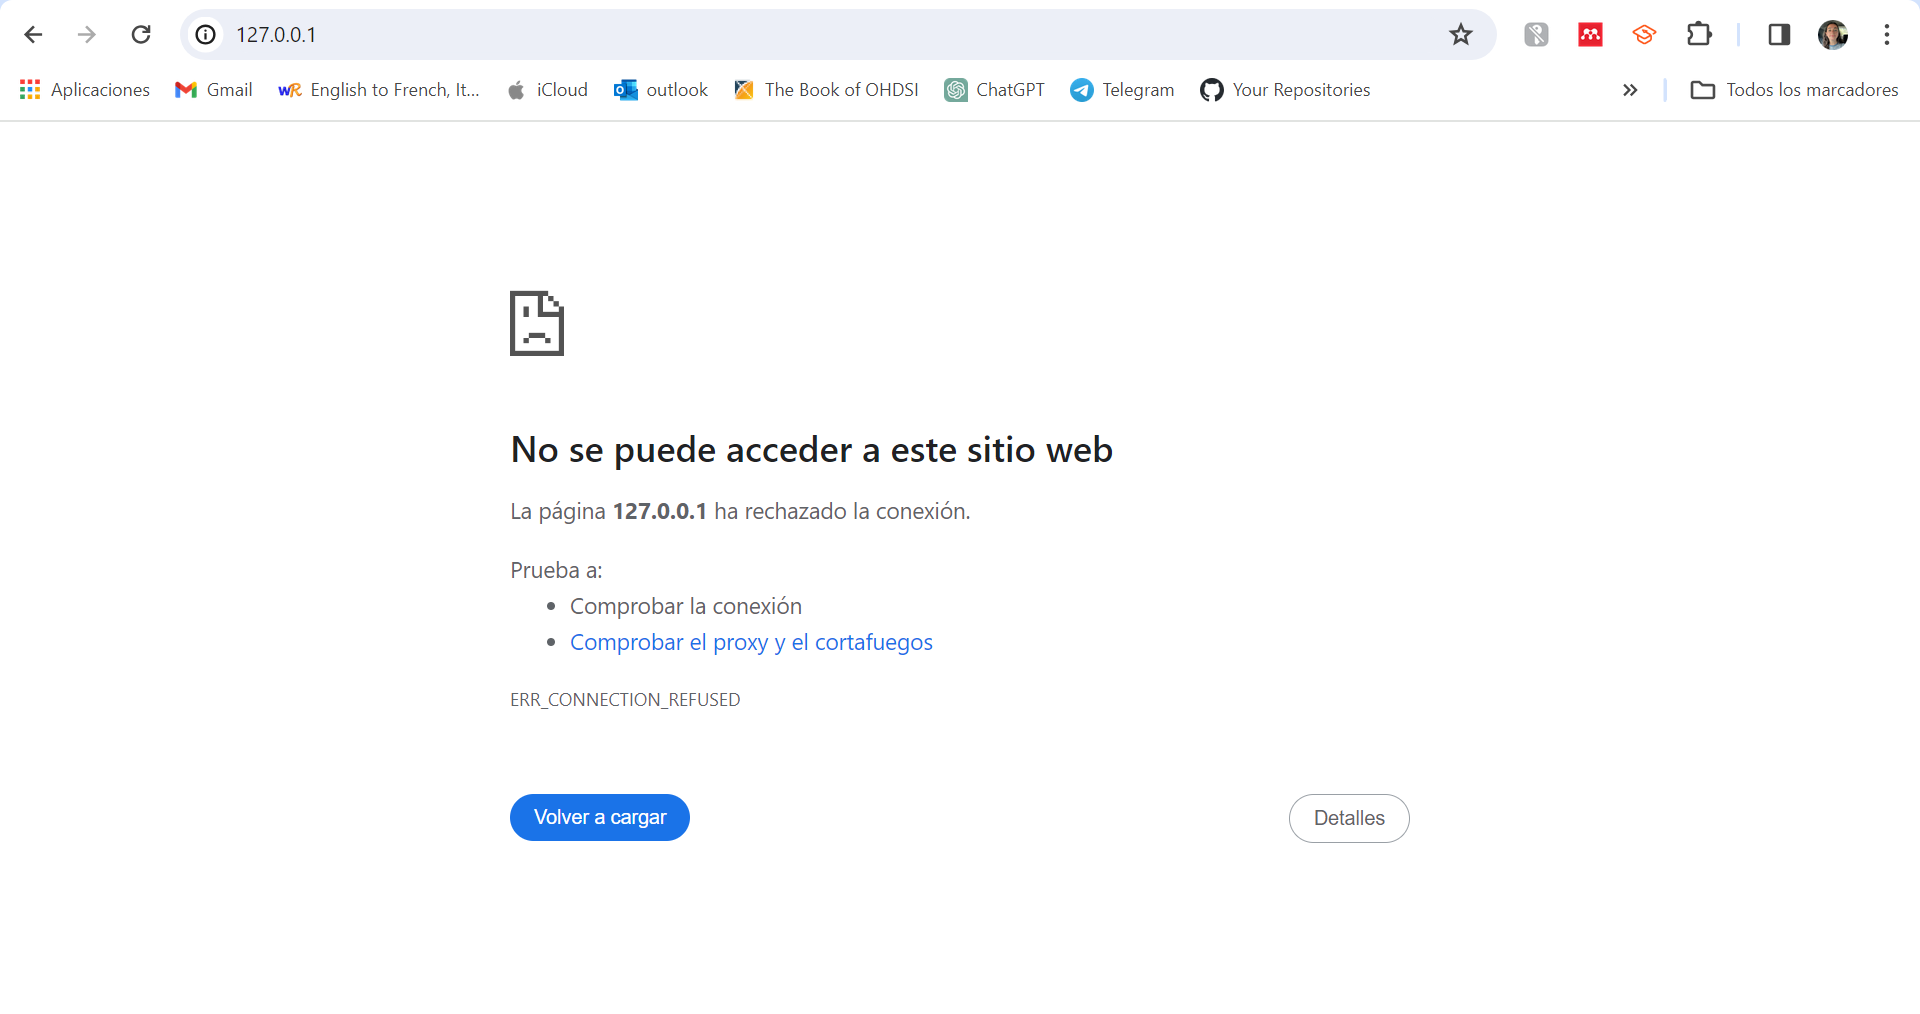
\includegraphics[width=0.90\textwidth]{figures/Error02NoSePuede.png}
     \caption{Captura de pantalla del error}
    \label{fig:Error02NoSePuede}
\end{figure}

Motivo: No se puede acceder al entorno Broadsea porque los contenedores Docker están detenidos.

Solución: Comprobar que todos los contenedores de docker implicados están corriendo. Para ello acceder a Docker Desktop y ejecutar todos los contenedores del multicontenedor de Broadsea. Una vez ejecutados todos los contenedores, si el problema persiste recargar varias veces la página.

\subsubsection{Error: Application initialization failed. Unable to connect to an instance of the WebAPI. Please contact your administrator to resolve this issue.}

Problema: Al abrir la herramienta ATLAS Broadsea aparece en rojo este error que impide conectar con la herramienta.

\begin{figure}[H]
    \centering
    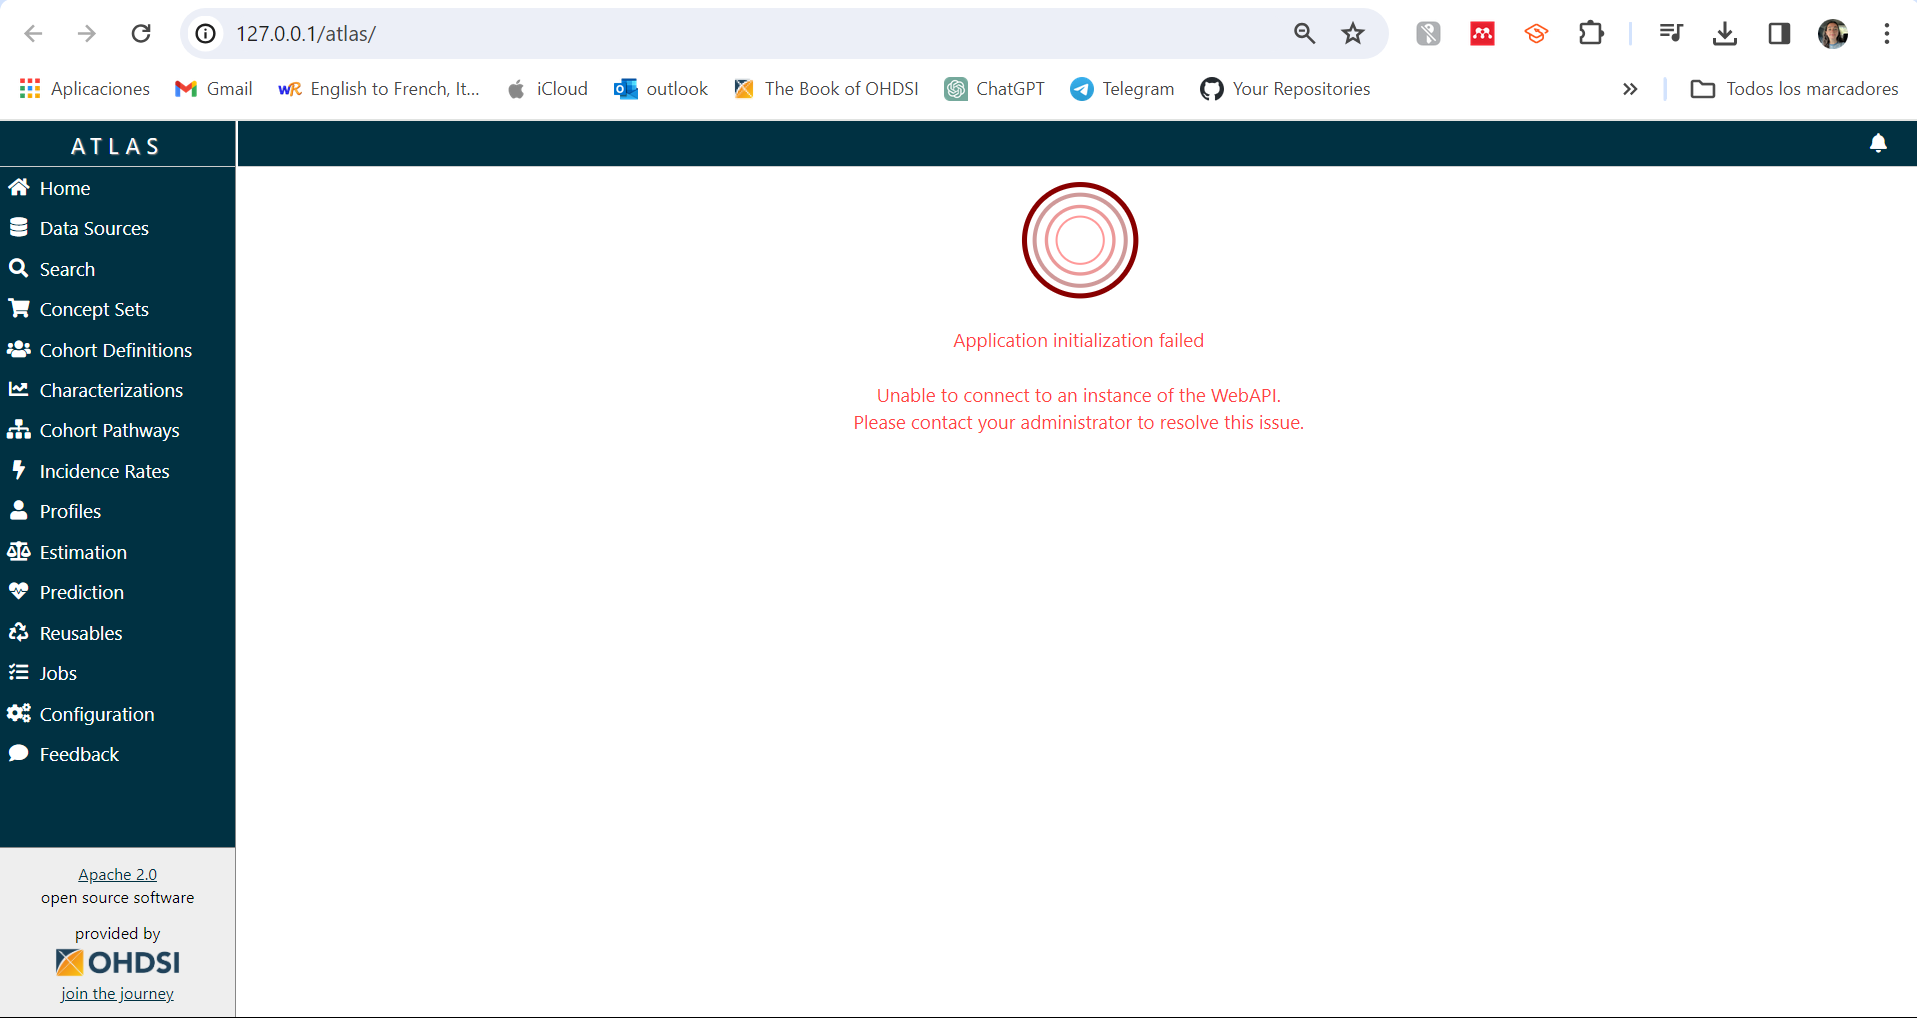
\includegraphics[width=0.90\textwidth]{figures/Error02AppFailed.png}
     \caption{Captura de pantalla del error}
    \label{fig:Error02AppFailed}
\end{figure}

Motivo: La aplicación falla al inicializarse porque no se está ejecutando correctamente el entorno docker de Broadsea.

Solución: Comprobar que todos los contenedores de docker implicados están corriendo. Para ello acceder a Docker Desktop y ejecutar todos los contenedores del multicontenedor de Broadsea. Una vez ejecutados todos los contenedores, si el problema persiste recargar varias veces la página.


